%===================================== CHAPTER 2 Pre-study =================================

\chapter{Pre-study}

This chapter discusses the research that had to be done, and the choices that the team made in relation to choosing development frameworks and technologies, as well as a development process for the project. The chapter also describes some already existing applications within the same subject as this one, and a study about personalization which was a key aspect for this project.

\section{Project assumptions and constraints}

In this section, assumptions and known constraints for the project are addressed. The list of assumptions are details assumed ahead of the documented project requirements, while the constraints specifies matters which would impact the project.

Assumptions on which the planning of the project was based:
\begin{itemize}
	\item Access to an  API for Digitalt fortalt would be provided by the customer.
	\item The customer would give access to a server to deploy the back end of the application on.
	\item The frameworks chosen for development had the features needed.
	\item The customer would be available for weekly meetings
	\item Each member of the team would be able to work about 20 hours a week.
	\item Team would meet at least three times a week.
	\item Team would follow the set ground rules.
\end{itemize}

Constraints which the team had to work within throughout the project:
\begin{itemize}
\item The deadline for delivering the project was May 30th, and there was no possibility to extend it.
\item The front end should be developed for both the iOS and Android platforms.
\item The team consisted of 7 people, with little previous experience in mobile app development and no knowledge of personalization algorithms.
\item The application is under the Apache license version 2.0 [HM7]. In summary, this grants copyright and patent rights for users to further distribute it, or distribute a modified version using the same license. It should be clear what the eventual modifications are. The source code can also be used as a part of a closed source project.
\item No budget to pay for software tools.
\end{itemize}

\section{Choice of framework}

As one of the requirements from the customer was that the application should be cross-platform (Android and iOS), a hybrid app was found to be the best option. The alternative would have been to create two separate native apps for both platforms. However, this would have been too much work to complete within the deadline, especially as the team had little experience with developing for either of the platforms. A hybrid app is a web app made with HTML and JavaScript wrapped in a native shell so that it can be run like a normal native app. This was a big advantage, as the team already had experience with web design. It also makes it possible to make use of the many tools available for web development, and most of the code can be reused for multiple platforms. Bad performance used to be a disadvantage to the hybrid approach, however mobile hardware has improved significantly in the last few years, so this is not a large issue any longer. The following sections will discuss the advantages and disadvantages of different frameworks that were considered, and explain the final choice for this project. \newline

\textbf{Table \ref{Tab:framework}} below summarizes some of the capabilities and limitations of the various frameworks that were under consideration.

\begin{table}[!h]
	\caption{Framework comparison}
		\begin{tabular}{ | p{6cm} | >{\raggedright}p{3cm} | >{\raggedright}p{3cm} | p{4cm} |}
			\hline
			\textbf{} & \textbf{PhoneGap w/ Ionic} & \textbf{Appcelerator Titanium} & \textbf{PhoneGap w/ Sencha Touch} \\ \hline
			\textbf{Can write a single code that runs on both iOS and Android?} & Yes & No & Yes \\ \hline
			\textbf{Access to native components} & Yes & Yes & Yes \\ \hline
			\textbf{Expected ease of learning and use} & Relatively easy & Difficult & Somewhat difficult \\ \hline
			\textbf{Performance of created application} & Good, AngularJS also provides a performance boost & Very good, as it provides direct access to native components & Acceptable, but not as performance- focused as Ionic. \\ \hline
			\textbf{Debugging} & Easy & Difficult & Easy \\ \hline
			\textbf{Programming language used} & HTML5, CSS, Javascript with AngularJS & Javascript & HTML5, CSS,\newline Javascript \\ \hline
		\end{tabular}
	\label{Tab:framework}
\end{table}

\subsection{PhoneGap}
\label{subsec:phonegap}

PhoneGap is an open-source mobile app framework for native packaging [RA2]. What it does is take in a mobile app consisting of HTML, CSS and JavaScript files, and wrap it in a native shell. It can then be deployed to iOS, Android and Windows 8. It also gives easy access to the native features of the phones (geolocation, notifications, storage, etc.) through different APIs. It is not necessary to think about the native SDKs, as the app will be compiled and built with the newest SDK for the platform.  It is a very popular framework, and there are many plugins created for it that provide additional functionality.

\subsection{Ionic}
\label{subsec:ionic}

Ionic is an open-source UI framework focused on making it easier to create hybrid mobile apps with a native feel [RA1]. It accomplishes this by offering a foundation to build on and UI components based on design patterns and best practices found in native apps. The foundation can be built on and customized with additional HTML, CSS and JavaScript. Part of the foundation is AngularJS, which is a JavaScript framework that extends HTML to make dynamic views in web applications. It gives the app a modular architecture, which means that code can more easily be reused for both iOS and Android. A disadvantage is that it is necessary to take time to learn AngularJS in order to take full advantage of Ionic. As Ionic is one of the most popular hybrid mobile frameworks, there exists more learning material about it, and it also has an active user community. Performance is not quite as good on older devices, especially if using large amounts of animations or media.

\subsection{Appcelerator Titanium}

Titanium is a cross-platform Javascript runtime and API framework [RA3]. It currently supports iOS and Android. It offers a JavaScript API which gives access to native UI components and features for the specific platforms, instead of trying to replicate it with CSS or JavaScript like other frameworks. This gives the app a performance advantage, and it is easier to make the interface and interactions feel native. Because the APIs are platform-specific you have to write separate versions of your app for the different platforms. Another disadvantage is that it is difficult to debug as there is no good debugger and Titanium projects cannot be run in Xcode. There would also have been more to learn to be able to use it, as it doesn’t use HTML/CSS.

\subsection{Sencha touch}

Sencha touch is a mobile framework with a large number of UI components and an architecture for the front end [RA4]. Instead of enhancing a HTML file, it generates the DOM with JavaScript. It can be used with PhoneGap, but Sencha also has its own native packager. It is harder to learn than Ionic, and the performance is not as good.  It supports the platforms iOS, Android, BlackBerry, and Windows Phone.

\subsection{Conclusion}

The framework combination chosen for this project was Ionic and PhoneGap, as this seemed to fit this project’s properties and requirements the best. They are both some of the most popular hybrid frameworks and they are a common combination to use. A prototype can quickly be set up with Ionic, and then iteratively customize it to fit the requirements and create a good user experience. One of the non-functional requirements was that it should be easy to extend the app and to reuse parts of it for other apps. This is fulfilled by Ionic’s modular structure. PhoneGap makes it easier to wrap the code in a native iOS and Android shell. This process could also have been done manually, but it requires some knowledge about the native code languages and SDKs. The many plugins available for PhoneGap should also cover the need for use of native features.

\section{Software development process}

The choice of which development process to use in the project was a central decision to be made. The following sections describe the different models that were under consideration by the team, as well as some advantages and disadvantages of each, which influenced the decision of which one to be used for the project. \textbf{Table \ref{Tab:dev-process}} below gives a comparison of some aspects of the various processes that were considered relevant for the project.

\begin{table}[!h]
	\begin{center}
		\caption{Development process comparison}
		\begin{tabular}{ | l | l | l | l |}
			\hline
			\textbf{} & \textbf{Scrum} & \textbf{Extreme Programming} & \textbf{Waterfall} \\ \hline
			\textbf{Type of methodology} & Agile & Agile & Plan-driven \\ \hline
			\textbf{Responds well to changes in requirements?} & Yes & Yes & No \\ \hline
			\textbf{Amount of planning needed} & Moderate & Very little & Very much \\ \hline
			\textbf{Level of detail for project plan} & Moderate & Low & High \\ \hline
			\textbf{Customer involvement} & High & High & Low \\ \hline
			\textbf{Frequency of testing} & Continuously & Continuously & Only near the end \\ \hline
			\textbf{Iteration length} & Short & Short & Long \\ \hline
		\end{tabular}
	\end{center}
	
	\label{Tab:dev-process}
\end{table}

\subsection{Waterfall model}
The waterfall model is a plan-driven process with well-defined phases. These phases normally include requirement analysis, system design, implementation, testing, and maintenance \cite[p.30-32]{Sommerville}. It is necessary to finish one phase before starting the next, and due to this, most planning and decisions need to be made at an early stage in the development. As such it is difficult to respond to changes in the requirements. Another issue with this model is that iterations often involve a significant amount of rework and it is normal to postpone some parts of the iterations in order to continue with the later stages of development. This can lead to errors in the system as well as bad design choices.

\subsection{Extreme programming}
Extreme programming is an agile method focused on pushing out new system versions and functionalities rapidly [es16 P.64-72]. All requirements are written as user scenarios, and before writing the code it is necessary to develop tests for the task. Team members program  in pairs and when the code passes all the tests, it can be integrated into the system.  It is common for a customer representative to take part in the development and make acceptance tests. New system releases are regularly presented to the customer, and this way it becomes easier to cope with changing requirements. Some of the drawbacks of extreme programming include the lack of overall plans for the project. Several documents such as design details and overall report are left out, and it lacks a solid plan for when to implement the various functionalities.


\subsection{Scrum }
\label{sec:scrum}
Scrum is a general agile method with focus on managing iterative development rather than specific technical engineering approaches [es16 P.72-74]. It also allows for a rapidly changing development environment and close collaboration between the members of a team. To provide this, scrum makes use of phases called sprints, daily scrum meetings, and several types of charts and logs. One of the main challenges for a scrum team is to choose the right amount of work per sprint so that they don’t end up with too little or too much work. Scrum has several similarities with extreme programming, such as high involvement of the customer in the development, as well as continuous testing while implementing new functionality.

\subsection{Conclusion}
For this project, the agile software development methodology scrum was used. The project was not very well defined from the beginning, because the customer was not entirely sure of exactly what they wanted. The team also became more productive, as the deadlines were short and so it was possible to quickly make a simple application which could be tested by users/customer. Also, an agile process was beneficial as it allowed the team to be flexible and rapidly respond to changes in requirements. The customer requested weekly meetings, and it became a logical decision to make use of scrum to have 1-week  sprints, so there would be definite progress to show between each customer meeting. Since the team was a group of seven, it was impossible to always work together. Because of this, the regular scrum meetings were beneficial to share and discuss progress.

\section{Back end}

\subsection{Docker}
\label{subsec:docker}

Docker[EHW2] was made to help automation of application deployment. This happens by providing a virtual operative-system-level abstraction. This means that on a server, it is possible to run several virtual operative systems called docker images, which can easily be deployed to another server. This is beneficial for software development, because it means it is easy to setup identical back ends. The customer used this on their servers, which made using it during development as well, a good choice. A benefit of using docker, is that it can directly access repositories on git. This means that the latest revision is guaranteed to run when starting the back end. However, there are also drawbacks. It is not possible to update files within the docker image currently running without rebuilding it. This means that to update a single line of code, the whole image needs to be rebuilt. This means that while the newest revision is guaranteed to be running, any changes made to the application after the start of that docker image requires manually stopping, rebuilding, and starting the docker image.

\subsection{Language}

\section{Personalization algorithms}
\label{sec:personalization_algorithms}

To provide story recommendations in accordance with each user’s interests the content needs to be personalized. Personalization involves using technology to tailor content, to individual users’ characteristics or preferences, and to accommodate the differences between individuals. It is a way of meeting the user’s needs by making interactions faster and easier, which will hopefully increase customer satisfaction and the likelihood of repeat visits. Personalization may be achieved using recommender systems.

\subsection{Recommender systems}

Recommender systems are software tools and techniques that attempts to provide recommendations of items [HM4]. Such systems are simply information filtering systems with the goal of providing suggestions for items to be of use or interest to a user. A few examples of items used in this context are movies, music, books and products in general. Recommender systems typically produce a list of recommendations.  The two most common approaches to produce such a list are content-based filtering and collaborative filtering.

\subsection{Content-based filtering}

Content-based filtering methods are used to find similarities between a user’s preferences and the description of an item [HM5]. These algorithms try to recommend items that are similar to items a user has liked in the past or is looking at in the present. Items that a user likes or has interacted with can be seen as a part of the user’s profile. Content-based filtering depends on there being much descriptive data available on the items. To find items to recommend, items are compared against a user’s profile, and recommendations are given based on how well they match the profile. User feedback, usually in the form of rating or a like or dislike button, can be used to assign weights to certain attributes. By using user feedback and weighting it is possible to give more accurate recommendations. [HM4]

\subsection{Collaborative filtering}

Collaborative filtering is based on collecting and comparing information on users’ behavior, activities or preferences and to recommend items based on a user’s similarity to other users [HM6]. This approach tries to predict what a user will like based on what similar users have liked. Collaborative filtering assumes that users who have agreed in the past will agree in the future, and that they will like similar items as they liked in the past. These methods often suffer from the problems cold start and sparsity. Collaborative filtering often requires a large amount of existing data on users to be able to make accurate recommendations. The cold start problem is the absence of such data at the beginning of a project. The sparsity problem is that collaborative systems are dependent on having many active users to properly distribute ratings across all the items in the system. However, most active users have only rated a few items in the overall database, which means that even the most popular items have very few ratings. The greatest strength of these techniques is that they are independent of any documented representation, e.g. textual descriptions and subject-tags, of the objects being recommended and work well for objects that are difficult to define such as music and movies. [HM4]

\section{Existing solutions}

Among the previous work there has been developed applications through the TagCloud project. This section evaluate two of those applications, namely stedr and Cooltura. Both of these applications presents stories regarding cultural heritage. Since this project also included personalization, an evaluation was additionally performed on the application Magic Tate Ball. This application was chosen because the customer mentioned this as a possible inspiration for the current project. \newline

These three applications were evaluated using the following criteria:
\begin{itemize}
\item Content. Does the application provide satisfying content or is something lacking?
\item Usability. Usability concerns how easy it is for the user to accomplish a task. (see \textbf{Section \ref{sec:non-functional_requirements}} for a more elaborate definition). The evaluation here draw on Jacob Nielsen’s ten usability heuristics as defined in \cite{AS3}.  
\item Personalization. To what extent does the application provide the user with the opportunity for individualized content?
\end{itemize}

The main findings in the evaluation are summarized in \textbf{Table \ref{Tab:existing_solutions}}.

\begin{table}[t]
	\caption{Summary of the main findings in the evaluation of existing solutions}
	\begin{tabular}[b]{ | p{2.7cm} | >{\raggedright}p{4.3cm} | >{\raggedright}p{4.3cm} | p{4.3cm} |}
		\hline
		\textbf{} & \textbf{stedr} & \textbf{Cooltura} & \textbf{Magic Tate Ball} \\ \hline
		\textbf{Content} & Stories related to places in Trondheim & Stories from three places, including Trondheim & Artworks and some information about them \\ \hline
		\textbf{Usability} & 
			- Requires knowledge of the location to find places on map \newline
			- The picture occupies much of the space in the place and story view \newline
			- Good help site\newline
			- Clear and consistent language 
			& 
			- List of locations is easier to navigate than a map and does not require knowledge of the exact location of the places\newline
			- Picture is dynamic and makes room for the relevant information to the user when scrolling \newline
			- Lacks a help site
			&  
			- Two options for starting the and for browsing the artworks accommodates different user groups \newline
			- Visibility of system status when processing 		
			 \\ \hline
		\textbf{Personalization} & Does not provide any personalization feature & Not implemented in the tested version & Provide personalization using different input parameters.  \\ \hline
	\end{tabular}
	\label{Tab:existing_solutions}
\end{table}

\subsection{stedr}
\label{subsec:stedr}

The stedr application was developed by students as a prototype to test some research hypothesis. Content was not the primary focus in the application and thus consists mainly of stories related to places in Trondheim. A possible problem in the application is finding the place the user is looking for since the main view consist of a map with markers representing each available place. In order to know which place each marker represents the user have to click on the marker, which means that the user might click on multiple markers do find the desired place. \newline 

The place view in stedr can be seen in \textbf{Figure \ref{Fig:stedr_screenshot}}. To see all the content, one might have to scroll down. The main picture is static when scrolling, occupying the upper half of the screen, which is also the case when viewing a specific story in the story view. It might be argued that Nielsen’s heuristic of aesthetic and minimalist design in case of scrolling is violated as the picture's importance in the dialogue is less important than the space it occupies suggest. \newline

\begin{figure}[h]
	\centering
	\begin{subfigure}[t]{0.3\textwidth}
		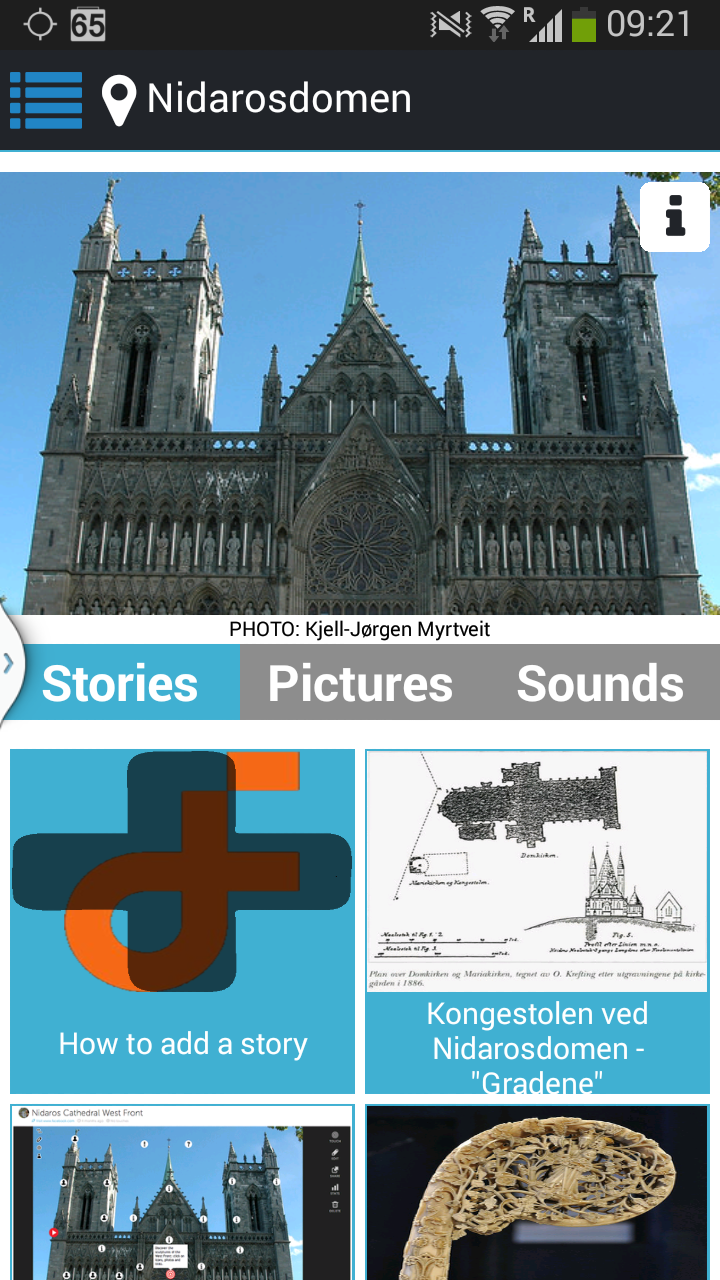
\includegraphics[width=\textwidth]{fig/stedr_screenshot}
		\caption{A screenshot from stedr showing the available options for one place}
		\label{Fig:stedr_screenshot}
	\end{subfigure}
	\hspace{0.5cm}
	\begin{subfigure}[t]{0.3\textwidth}
		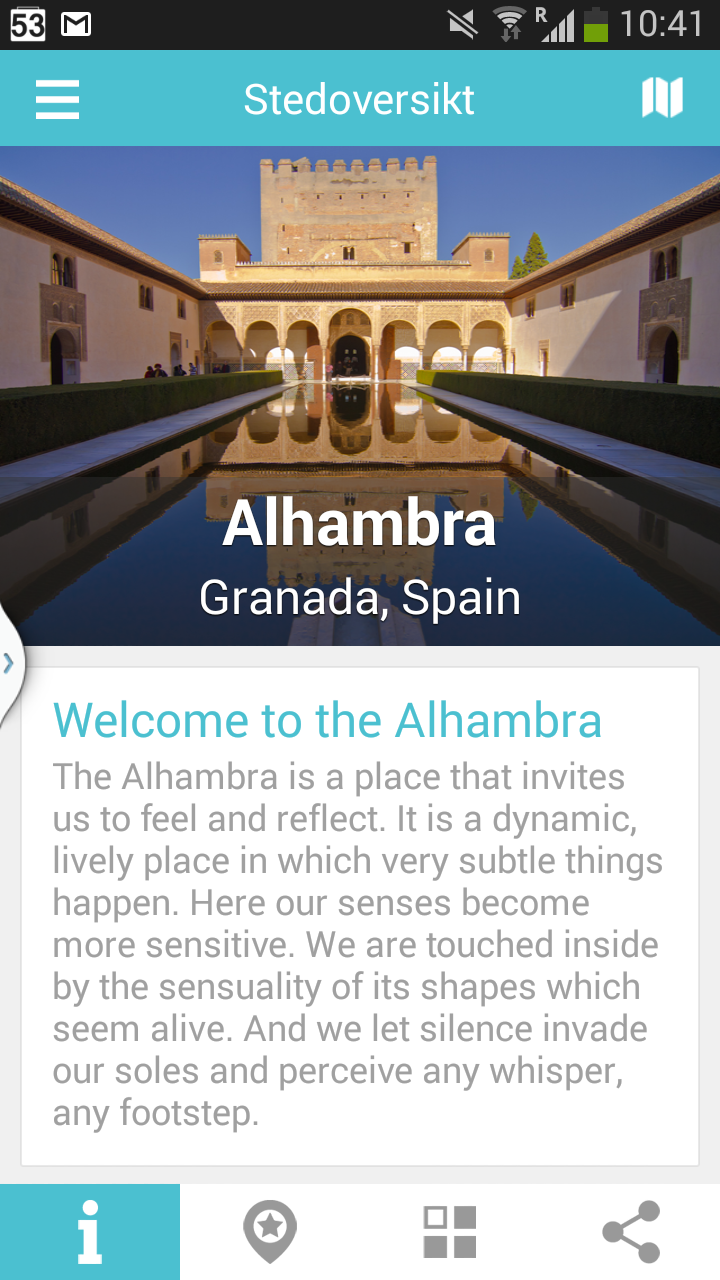
\includegraphics[width=\textwidth]{fig/cooltura_screenshot2}
		\caption{A screenshot of Cooltura showing the view for one particular place}
		\label{Fig:cooltura_screenshot2}	
	\end{subfigure}	
	\hspace{0.5cm}	
	\begin{subfigure}[t]{0.3\textwidth}
		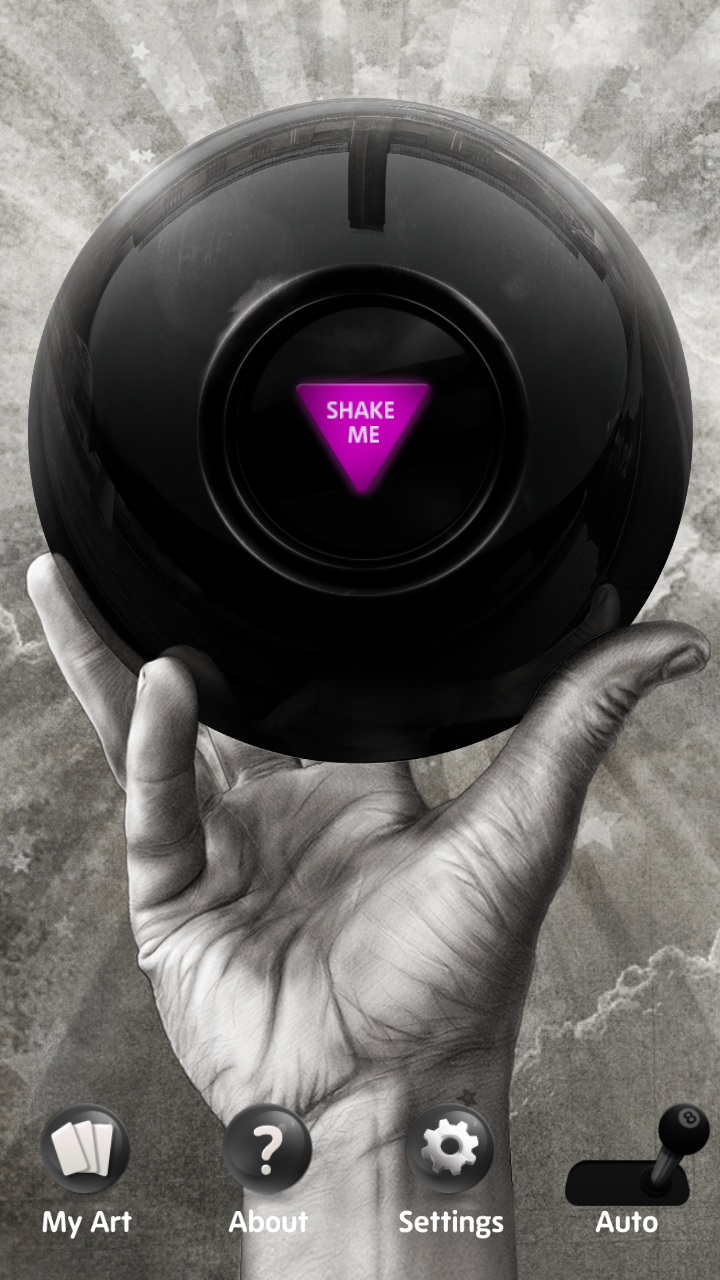
\includegraphics[width=\textwidth]{fig/tateball_screenshot}
		\caption{A screenshot of the main view of Magic Tate Ball}
		\label{Fig:tateball_screenshot}		
	\end{subfigure}	
	\caption{Place views in stedr and Cooltura and the main view of Magic Tate Ball}
\end{figure}

The application provides a help site which gives a thorough guide to the user on how to accomplish tasks. This is in accordance with Nielsen’s heuristic of help and documentation. The application also helps the user when errors occur, for instance by offering the user a refresh opportunity when the map does not load the places. The language used in the application is both user-centered and consistent, avoiding misunderstandings and making it easy for the user to understand what different actions entails. \newline

The application does not provide any personalization feature, which is the main difference between stedr and our application. The customer’s motivation for creating an entirely new application instead of expanding stedr was mainly because they wished to test personalization systems on users, and thus needed an application focused mainly around the personalization aspect. In addition, it became possible to access a larger number of stories than stedr currently does. 

\subsection{Cooltura}

Cooltura is another application developed under the TagCloud umbrella. The version of Cooltura evaluated here is a demo version, so more developed versions of the application may include more functionality and address some of the issues discussed here. \newline

The content is somewhat similar to stedr, with respect to the places and the stories available. In fact, when clicking to view stories in Cooltura one is directed to the stedr app. Cooltura does not use a map like stedr, but instead a list of available locations. This makes it far easier for the user to navigate to the right place, especially since the selection is quite limited. When viewing a specific place on Cooltura the user gets a view with a main picture and some text describing the place as seen in \textbf{Figure \ref{Fig:cooltura_screenshot2}}. Like in stedr the user can scroll down to see more content, but unlike stedr the main picture is not static, that is, the user see less and less of it as it scrolls down. This is more in accordance with Nielsen’s point of aesthetic and minimalist design, where less relevant information fills up less space in the user interface. The same is true for the view for a specific tourist attraction. The application does not provide any help site, but the possible user actions are quite few and similar (most of them are about navigating to the desired place), so this might not be a problem.\newline

It appears that the application intends to make use of personalization, but this is not implemented at the time of writing this report \cite{AS4}. The “Anbefalte steder”-view in Cooltura now list every place added in the application (which is three different places), but the heading suggests that personalization is planned for. 

\subsection{Magic Tate Ball}

Magic Tate Ball is an application that presents the user with an artwork based on the input parameters: date, time-of-day, geographical location, live weather data and ambient noise levels \cite{AS5}. The content in the application is the artwork, a description of the artwork and an explanation of why the artwork was chosen. Personalization is the main selling point of Magic Tate Ball. The application uses the input parameters to give the user some control of what content is presented as the user can turn each of these parameters on and off. Even though the application provides an explanation to why an artwork was chosen, how it was chosen remains in the dark (e.g. how to know which input parameter was emphasized in the personalization).\newline


The main task in the application is to be presented with an artwork. This is done by shaking the phone or by clicking a button in the center of the magic ball, see \textbf{Figure \ref{Fig:tateball_screenshot}} for a screenshot of this. Another task is to browse all artworks presented to the user, which is done by swiping or clicking on arrows. Providing these two options makes it easy to for different types of users, those accustomed to swiping and those who are not. When the application is processing to come up with an artwork to present to the user, it shows the user what the input parameters are. This is in accordance with Nielsen’s heuristics on visibility of system status. \newline

\cleardoublepage